%-----------------------------------------------------------------------------%
\chapter{LANDASAN TEORI}
%-----------------------------------------------------------------------------%

%
\vspace{4.5pt}

\begin{flushleft}
    \section{Tinjauan Pustaka}
    \section{Dasar Teori}
    \begin{justify}
        \subsection{\textit{Monitoring} dan Kontrol}
        Menurut Dr. Harry Hikmat (2010), monitoring adalah proses pengumpulan
dan analisis informasi berdasarkan indikator yang ditetapkan secara sistematis dan
berkelanjutan tentang kegiatan/program sehingga dapat dilakukan tindakan
koreksi untuk penyempurnaan program/kegiatan itu selanjutnya
Sistem kontrol atau
sistem kendali adalah kumpulan dari beberapa komponen yang terhubung satu
sama lainnya, sehingga membentuk suatu tujuan tertentu yaitu mengendalikan
atau mengatur suatu sistem (Ogata, 1997). 
\\

        \subsection{Aplikasi \textit{Mobile}}
        Aplikasi \textit{mobile} adalah program perangkat lunak yang dirancang untuk dijalankan di smartphone, tablet, dan perangkat lain [N. Serrano]. Urgensi penggunaan Aplikasi yang dikembangkan berbasis mobile adalah semakin meningkatnya pengguna smartphone yang membutuhkan berbagai macam alat sebagai fasilitator dalam kegiatan sehari-hari. Sebagai fasilitator, aplikasi mobile harus mampu menyediakan informasi agar dapat menjadi sumber data bagi penggunanya dan mampu meningkatkan produktifitas pengguna. 
        \\
        \subsection{\textit{Rapid Application Development} (RAD)}
        Dalam referensi [\textbf{SUMBER}] terdapat lima tahapan dalam model RAD : (1) Pemodelan bisnis, (2) Pemodelan data, (3) Pemodelan proses, (4) Pembentukan aplikasi, (5) Pengujian dan \textit{turnover} .
        
        \begin{figure}[ht]
            \centering
           
	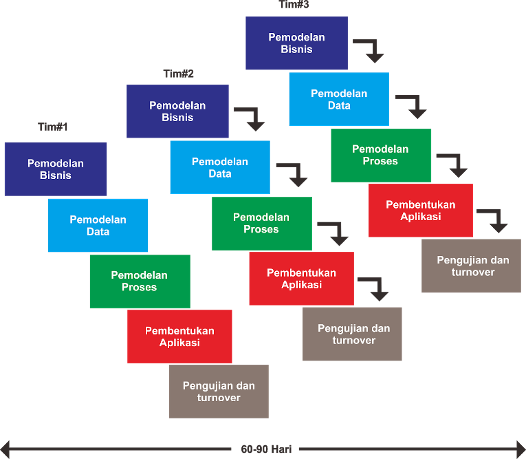
\includegraphics[width=6cm]{images/RAD.png}\\
            \caption{Gambar Ilustrasi Model RAD}
        \end{figure}
        Berdasarkan Gambar 3, dapat diperhatikan penjabaran sebagai berikut :
        \begin{enumerate}[label=\alph*.]
            \item Pemodelan Bisnis\\
            Pada tahap ini output yang dihasilkan berupa dokumen \textit{Software Requirements Specification} (SRS) yang meliputi informasi ketentuan aplikasi yang akan dibuat. Dokumen tersebut mencakup informasi apa saja yang harus dibuat, siapa yang harus membuat informasi itu, bagaimana alur informasi itu, proses apa saja yang terkait informasi itu.
            \item Pemodelan Data\\
            Memodelkan data apa saja yang dibutuhkan berdasarkan pemodelan bisnis dan mendefinisikan atribut-atributnya beserta relasinya dengan data-data yang lain. 
            \item Pemodelan Proses\\
            Mengimplementasikan fungsi bisnis yang sudah didefinisikan terkait dengan pendefinisian data. 
            \item Pembuatan Aplikasi\\
            Mengimplementasikan pemodelan proses dan data menjadi program. Model RAD sangat menganjurkan pemakaian komponen yang sudah ada jika dimungkinkan.
            \item Pengujian dan Pergantian\\
            Menguji komponen-komponen yang dibuat. Jika sudah teruji maka tim pengembang komponen dapat beranjak untuk mengembangkan komponen berikutnya.\\
        \end{enumerate}

        \subsection{Flutter}
        Flutter merupakan sebuah framework aplikasi mobile yang bersifat open source (terbuka) yang diciptakan oleh Google. Flutter dapat digunakan dalam pengembangan aplikasi mobile untuk sistem operasi Android dan iOS, bahkan juga dapat digunakan dalam pengembangan Web ataupun Desktop dari codebase tunggal. Flutter merupakan framework dengan penggunaan Bahasa Dart.
Berikut ini bebrapa kelebihan dari Flutter [\textbf{SUMBER}] :
\begin{enumerate}
    \item \textit{Package modules} sudah terkoneksi secara otomatis di dalam flutter, sehingga tidak terlalu repot untuk memanggil secara manual melalui terminal
    \item Dart menggunakan konsep OOP (\textit{Object Orinented Programming})
    \item \textit{Setup} secara manual jauh lebih mudah, apabila kita memerlukan \textit{library} baru, cukup tambahkan di bagian puspec.yaml
    \item Performa cepat dan  \textit{smooth}
    \item Data management menggunakan state sehingga lebih mudah dalam penggunaannya
    \item Adanya fitur \textit{Hot Reload} yang membantu debug lebih cepat
    \item Disupport oleh IDE yang sudah familiar dikalangan developer android, seperti Android Studio dan Visual Code\\
    
\end{enumerate}


        \subsection{\textit{Application Programming Interface} (API)}
            \textit{Application Programming Interface} atau API memungkinkan perusahaan untuk membuka data dan fungsionalitas aplikasi mereka kepada pengembang pihak ketiga eksternal, mitra bisnis, dan departemen internal di dalam perusahaan mereka. Hal ini memungkinkan layanan dan produk untuk berkomunikasi satu sama lain dan memanfaatkan data dan fungsionalitas satu sama lain melalui antarmuka yang terdokumentasi. Pengembang tidak perlu tahu bagaimana API diimplementasikan; mereka hanya menggunakan antarmuka untuk berkomunikasi dengan produk dan layanan lain. Penggunaan API telah melonjak selama dekade terakhir, sampai pada tingkat di mana banyak aplikasi web paling populer saat ini tidak akan mungkin tanpa API.


        \subsection{Database}

        \subsection{\textit{Flowchart}}

        \subsection{\textit{Use Case} Diagram}

        \subsection{\textit{Black Box Testing}}

        \subsection{\textit{User Acceptance Testing} (UAT)}
        \noindent User Acceptance Testing (UAT) adalah pengujian terakhir yang dilakukan oleh user secara langsung, dan pada saat pengujian berlangsung pembuatan dokumen juga dilakukan sebagai bukti penerimaan sistem oleh pengguna. 
        \textcolor{red}{[Mutiara, A. B., Awaludin, R., Muslim, A. and T. Oswari, “Testing Implementasi Website Rekam Medis Elektronik Opeltgunasys Dengan Metode Acceptance Testing,” 2014.].
        }
        

        \subsection{Skala \textit{Likert}}

    \end{justify}



\end{flushleft}



\newpage